% -*- TeX-engine: xetex; eval: (auto-fill-mode 0); eval: (visual-line-mode 1); -*-
% Compile with XeLaTeX

%%%%%%%%%%%%%%%%%%%%%%%
% Option 1: Slides: (comment for handouts)   %
%%%%%%%%%%%%%%%%%%%%%%%

\documentclass[slidestop,compress,mathserif,12pt,t,professionalfonts,xcolor=table]{beamer}

% solution stuff
\newcommand{\solnMult}[1]{
\only<1>{#1}
\only<2->{\red{\textbf{#1}}}
}
\newcommand{\soln}[1]{\textit{#1}}

%%%%%%%%%%%%%%%%%%%%%%%%%%%%%%%
% Option 2: Handouts, without solutions (post before class)    %
%%%%%%%%%%%%%%%%%%%%%%%%%%%%%%%

% \documentclass[11pt,containsverbatim,handout,xcolor=xelatex,dvipsnames,table]{beamer}

% % handout layout
% \usepackage{pgfpages}
% \pgfpagesuselayout{4 on 1}[letterpaper,landscape,border shrink=5mm]

% % solution stuff
% \newcommand{\solnMult}[1]{#1}
% \newcommand{\soln}[1]{}

% % % This breaks things for me for some reason.
% % tell pgfpages how to set page sizes in XeLaTeX
% %\renewcommand\pgfsetupphysicalpagesizes{%
% %   \pdfpagewidth\pgfphysicalwidth\pdfpageheight\pgfphysicalheight%
% %}

%%%%%%%%%%%%%%%%%%%%%%%%%%%%%%%%%%%%
% Option 3: Handouts, with solutions (may post after class if need be)    %
%%%%%%%%%%%%%%%%%%%%%%%%%%%%%%%%%%%%

% \documentclass[11pt,containsverbatim,handout,xcolor=xelatex,dvipsnames,table]{beamer}

% % handout layout
% \usepackage{pgfpages}
% \pgfpagesuselayout{4 on 1}[letterpaper,landscape,border shrink=5mm]

% % solution stuff
% \newcommand{\solnMult}[1]{\red{\textbf{#1}}}
% \newcommand{\soln}[1]{\textit{#1}}

% % % This breaks things for me for some reason.
% % % tell pgfpages how to set page sizes in XeLaTeX
% % \renewcommand\pgfsetupphysicalpagesizes{%
% %    \pdfpagewidth\pgfphysicalwidth\pdfpageheight\pgfphysicalheight%
% % }

%%%%%%%%%%%%%%%%%%%%%%%%%%%%%%%
% Option 4: Notes Only
%%%%%%%%%%%%%%%%%%%%%%%%%%%%%%%

% % See http://tex.stackexchange.com/questions/114219/add-notes-to-latex-beamer
% \documentclass[10pt,containsverbatim,xcolor=xelatex,dvipsnames,table,notes=only]{beamer}

% % handout layout
% \usepackage{pgfpages}
% \pgfpagesuselayout{2 on 1}[letterpaper, landscape, border shrink=5mm]

% % solution stuff
% \newcommand{\solnMult}[1]{#1}
% \newcommand{\soln}[1]{}

% % % Having a problem with this.
% % tell pgfpages how to set page sizes in XeLaTeX
% % \renewcommand\pgfsetupphysicalpagesizes{%
% %   \pdfpagewidth\pgfphysicalwidth\pdfpageheight\pgfphysicalheight%
% %}

%%%%%%%%%%
% Load style file, defaults  %
%%%%%%%%%%

%%%%%%%%%%%%%%%%
% Themes
%%%%%%%%%%%%%%%%

% See http://deic.uab.es/~iblanes/beamer_gallery/ for mor options

% Style theme
\usetheme{Pittsburgh}

% Color theme
\usecolortheme{seahorse}

% Helvetica Neue Light for most text
\usepackage{fontspec}
\setsansfont{Helvetica Neue Light}

%%%%%%%%%%%%%%%%
% Packages
%%%%%%%%%%%%%%%%

\usepackage{geometry}
\usepackage{graphicx}
\usepackage{amssymb}
\usepackage{epstopdf}
\usepackage{amsmath}  	% this permits text in eqnarray among other benefits
\usepackage{url}		% produces hyperlinks
\usepackage[english]{babel}
\usepackage{colortbl}	% allows for color usage in tables
\usepackage{multirow}	% allows for rows that span multiple rows in tables
\usepackage{color}		% this package has a variety of color options
\usepackage{pgf}
\usepackage{calc}
\usepackage{ulem}
\usepackage{multicol}
\usepackage{textcomp}
\usepackage{listings}
\usepackage{changepage}
\usepackage{tikz}
\usetikzlibrary{trees}		% for probability trees
\usepackage{fancyvrb}	% for colored code chunks
\usepackage{nameref}

%%%%%%%%%%%%%%%%
% Remove navigation symbols
%%%%%%%%%%%%%%%%

\beamertemplatenavigationsymbolsempty
\hypersetup{pdfpagemode=UseNone} % don't show bookmarks on initial view

%%%%%%%%%%%%%%%%
% User defined colors
%%%%%%%%%%%%%%%%

% Pantone 2015 Fall colors
% http://iwork3.us/2015/02/18/pantone-2015-fall-fashion-report/
% update each semester or year

\xdefinecolor{custom_blue}{rgb}{0, 0.32, 0.48} % FROM SPRING 2016 COLOR PREVIEW
\xdefinecolor{custom_darkBlue}{rgb}{0.20, 0.20, 0.39} % Reflecting Pond  
\xdefinecolor{custom_orange}{rgb}{0.96, 0.57, 0.42} % Cadmium Orange
\xdefinecolor{custom_green}{rgb}{0, 0.47, 0.52} % Biscay Bay
\xdefinecolor{custom_red}{rgb}{0.58, 0.32, 0.32} % Marsala

\xdefinecolor{custom_lightGray}{rgb}{0.78, 0.80, 0.80} % Glacier Gray
\xdefinecolor{custom_darkGray}{rgb}{0.35, 0.39, 0.43} % Stormy Weather

%%%%%%%%%%%%%%%%
% Template colors
%%%%%%%%%%%%%%%%

\setbeamercolor*{palette primary}{fg=white,bg= custom_blue}
\setbeamercolor*{palette secondary}{fg=black,bg= custom_blue!80!black}
\setbeamercolor*{palette tertiary}{fg=white,bg= custom_blue!80!black!80}
\setbeamercolor*{palette quaternary}{fg=white,bg= custom_blue}

\setbeamercolor{structure}{fg= custom_blue}
\setbeamercolor{frametitle}{bg= custom_blue!90}
\setbeamertemplate{blocks}[shadow=false]
\setbeamersize{text margin left=2em,text margin right=2em}

%%%%%%%%%%%%%%%%
% Styling fonts, bullets, etc.
%%%%%%%%%%%%%%%%

% title slide
\setbeamerfont{title}{size=\large,series=\bfseries}
\setbeamerfont{subtitle}{size=\large,series=\mdseries}
%\setbeamerfont{institute}{size=\large,series=\mdseries}

% color of alerted text
\setbeamercolor{alerted text}{fg=custom_orange}

% styling of itemize bullets
\setbeamercolor{item}{fg=custom_blue}
\setbeamertemplate{itemize item}{{{\small$\blacktriangleright$}}}
\setbeamercolor{subitem}{fg=custom_blue}
\setbeamertemplate{itemize subitem}{{\textendash}}
\setbeamerfont{itemize/enumerate subbody}{size=\footnotesize}
\setbeamerfont{itemize/enumerate subitem}{size=\footnotesize}

% styling of enumerate bullets
\setbeamertemplate{enumerate item}{\insertenumlabel.}
\setbeamerfont{enumerate item}{family={\fontspec{Helvetica Neue}}}
\setbeamerfont{enumerate subitem}{family={\fontspec{Helvetica Neue}}}
\setbeamerfont{enumerate subsubitem}{family={\fontspec{Helvetica Neue}}}

% make frame titles small to make room in the slide
\setbeamerfont{frametitle}{size=\small} 

% set Helvetica Neue font for frame and section titles
\setbeamerfont{frametitle}{family={\fontspec{Helvetica Neue}}}
\setbeamerfont{sectiontitle}{family={\fontspec{Helvetica Neue}}}
\setbeamerfont{section in toc}{family={\fontspec{Helvetica Neue}}}
\setbeamerfont{subsection in toc}{family={\fontspec{Helvetica Neue}}, size=\small}
\setbeamerfont{footline}{family={\fontspec{Helvetica Neue}}}
\setbeamerfont{subsection in toc}{family={\fontspec{Helvetica Neue}}}
\setbeamerfont{block title}{family={\fontspec{Helvetica Neue}}}

%%%%%%%%%%%%%%%%
% New fonts accessed by fontspec package
%%%%%%%%%%%%%%%%

% Monaco font for code
\newfontfamily{\monaco}{Monaco}

%%%%%%%%%%%%%%%%
% Color text commands
%%%%%%%%%%%%%%%%

%orange
\newcommand{\orange}[1]{\textit{\textcolor{custom_orange}{#1}}}

% yellow
\newcommand{\yellow}[1]{\textit{\textcolor{yellow}{#1}}}

% blue
\newcommand{\blue}[1]{\textit{\textcolor{blue}{#1}}}

% green
\newcommand{\green}[1]{\textit{\textcolor{custom_green}{#1}}}

% red
\newcommand{\red}[1]{\textit{\textcolor{custom_red}{#1}}}

% dark gray
\newcommand{\darkgray}[1]{\textit{\textcolor{custom_darkGray}{#1}}}

% light gray
\newcommand{\lightgray}[1]{\textit{\textcolor{custom_lightGray}{#1}}}

% pink
\newcommand{\pink}[1]{\textit{\textcolor{pink}{#1}}}


%%%%%%%%%%%%%%%%
% Custom commands
%%%%%%%%%%%%%%%%

% empty box for probability tree frame
\newcommand{\emptybox}[2]{
	\fbox{ \begin{minipage}{#1} \hfill\vspace{#2} \end{minipage} }
}

% cancel
\newcommand{\cancel}[1]{%
    \tikz[baseline=(tocancel.base)]{
        \node[inner sep=0pt,outer sep=0pt] (tocancel) {#1};
        \draw[red, line width=0.5mm] (tocancel.south west) -- (tocancel.north east);
    }%
}

% degree
\newcommand{\degree}{\ensuremath{^\circ}}

% cite
\newcommand{\ct}[1]{
\vfill
{\tiny #1}}

% Note
\newcommand{\Note}[1]{
\rule{2.5cm}{0.25pt} \\ \textit{\footnotesize{\textcolor{custom_red}{Note:} \textcolor{custom_darkGray}{#1}}}}

% Remember
\newcommand{\Remember}[1]{\textit{\scriptsize{\textcolor{custom_red}{Remember:} #1}}}

% links: webURL, webLink
\newcommand{\webURL}[1]{\urlstyle{same}{\textit{\textcolor{custom_blue}{\url{#1}}}}}
\newcommand{\webLink}[2]{\href{#1}{\textcolor{custom_blue}{{#2}}}}

% mail
\newcommand{\mail}[1]{\href{mailto:#1}{\textit{\textcolor{custom_blue}{#1}}}}

% highlighting: hl, hlGr, mathhl
\newcommand{\hl}[1]{\textit{\textcolor{custom_blue}{#1}}}
\newcommand{\hlGr}[1]{\textit{\textcolor{custom_green}{#1}}}
\newcommand{\mathhl}[1]{\textcolor{custom_blue}{\ensuremath{#1}}}

% example
\newcommand{\ex}[1]{\textcolor{blue}{{{\small (#1)}}}}

% two col: two columns
\newenvironment{twocol}[4]{
\begin{columns}[c]
\column{#1\textwidth}
#3
\column{#2\textwidth}
#4
\end{columns}
}

% slot (for probability calculations)
\newenvironment{slot}[2]{
\begin{array}{c} 
\underline{#1} \\ 
#2
\end{array}
}

% pr: left and right parentheses
\newcommand{\pr}[1]{
\left( #1 \right)
}

%%%%%%%%%%%%%%%%
% Custom blocks
%%%%%%%%%%%%%%%%

% activity: less commonly used
\newcommand{\activity}[2]{
\setbeamertemplate{itemize item}{{{\small\textcolor{custom_orange}{$\blacktriangleright$}}}}
\setbeamercolor{block title}{fg=white, bg=custom_orange}
\setbeamerfont{block title}{size=\small}
\setbeamercolor{block body}{fg=black, bg=custom_orange!20!white!80}
\setbeamerfont{block body}{size=\small}
\begin{block}{Activity: #1}
\setlength\abovedisplayskip{0pt}
#2
\end{block}
}

% app: application exercise
\newcommand{\app}[2]{
\setbeamercolor{block title}{fg=white,bg=custom_green}
\setbeamercolor{block body}{fg=black,bg=custom_green!20!white!80}
\begin{block}{{\small Application exercise: #1}}
#2
\end{block}
}

% disc: discussion question
\newcommand{\disc}[1]{
\vspace*{-2ex}
\setbeamercolor{block body}{bg=custom_blue!25!white!80, fg=custom_blue!55!black!95}
\begin{block}{\vspace*{-3ex}}
#1
\end{block}
\vspace*{-1ex}
}

% clicker: clicker question
\newcommand{\clicker}[1]{
\setbeamercolor{block title}{bg=custom_blue!80!white!50,fg=custom_blue!30!black!90}
\setbeamercolor{block body}{bg=custom_blue!20!white!80,fg=custom_blue!30!black!90}
\begin{block}{\vspace*{-0.2ex}{\footnotesize Clicker question}\vspace*{-0.2ex}}
#1
\end{block}
}

% formula
\newcommand{\formula}[2]{
\setbeamercolor{block title}{bg=custom_blue!40!white!60,fg=custom_blue!55!black!95}
\begin{block}{{\small#1}}
#2
\end{block}
}

% code
\newcommand{\Rcode}[1]{
{\monaco {\footnotesize \textcolor{custom_darkBlue}{#1}}}
}

% output
\newcommand{\Rout}[1]{
{\monaco {\footnotesize \textcolor{custom_darkGray}{#1}}}
}

%%%%%%%%%%%%%%%%
% Change margin
%%%%%%%%%%%%%%%%

\newenvironment{changemargin}[2]{%
\begin{list}{}{%
\setlength{\topsep}{0pt}%
\setlength{\leftmargin}{#1}%
\setlength{\rightmargin}{#2}%
\setlength{\listparindent}{\parindent}%
\setlength{\itemindent}{\parindent}%
\setlength{\parsep}{\parskip}%
}%
\item}{\end{list}}

%%%%%%%%%%%%%%%%
% Footnote
%%%%%%%%%%%%%%%%

\long\def\symbolfootnote[#1]#2{\begingroup%
\def\thefootnote{\fnsymbol{footnote}}\footnote[#1]{#2}\endgroup}

%%%%%%%%%%%%%%%%
% Graphics
%%%%%%%%%%%%%%%%

\DeclareGraphicsRule{.tif}{png}{.png}{`convert #1 `dirname #1`/`basename #1 .tif`.png}

%%%%%%%%%%%%%%%%
% Slide number
%%%%%%%%%%%%%%%%

\setbeamertemplate{footline}{%
    \raisebox{5pt}{\makebox[\paperwidth]{\hfill\makebox[20pt]{\color{gray}
          \scriptsize\insertframenumber}}}\hspace*{5pt}}

          
%%%%%%%%%%%%%%%%
% Remove page numbers
%%%%%%%%%%%%%%%%

\newcommand{\removepagenumbers}{% 
  \setbeamertemplate{footline}{}
}

%%%%%%%%%%%%%%%%
% TOC slides
%%%%%%%%%%%%%%%%

\setbeamertemplate{section in toc}{\inserttocsectionnumber.~\inserttocsection}
\setbeamertemplate{subsection in toc}{$\qquad$\inserttocsubsectionnumber.~\inserttocsubsection \\}

\AtBeginSection[] 
{ 
  \addtocounter{framenumber}{-1} 
  % 
  {\removepagenumbers 
  {\small
    \begin{frame}<beamer> 
    \frametitle{Outline} 
    \tableofcontents[currentsection] 
  \end{frame} 
  } 
  }
} 

\AtBeginSubsection[] 
{ 
  \addtocounter{framenumber}{-1} 
  % 
  {\removepagenumbers 
  {\small
    \begin{frame}<beamer> 
    \frametitle{Outline} 
    \tableofcontents[currentsection,currentsubsection] 
  \end{frame} 
  } 
  }
}
% You cannot use numbers when defining variables.  
% Hence the use of letters, A, B, C, etc.

% Course Name
\newcommand{\CourseName}{Sta 101 - Fall 2015}
\newcommand{\InstituteName}{Duke University, Department of Statistical Science}

% Personal Info
\newcommand{\FirstName}{Mine}
\newcommand{\LastName}{\c{C}etinkaya-Rundel}
\newcommand{\OfficeHours}{Tue + Thur 4:30-6pm}
\newcommand{\OfficeHoursLocation}{Old Chem 213}

% Electronic Info
\newcommand{\PersonalSite}{http://stat.duke.edu/~mc301}
\newcommand{\CourseSite}{http://bit.ly/sta101_f15}
\newcommand{\Email}{mine@stat.duke.edu}

% TAs
\newcommand{\TAA}{Erika Ball}
\newcommand{\TAB}{David Clancy}
\newcommand{\TAC}{Reuben McCreanor}
\newcommand{\TAD}{Anne Driscoll}
\newcommand{\TAE}{Megan Robertson}

% Exam Dates
\newcommand{\ExamADate}{Mon, Oct 5}
\newcommand{\ExamBDate}{Mon, Nov 9}
\newcommand{\FinalDate}{Thur, Dec 10 (2-5pm)}


% ALT ALT
% % You cannot use numbers when defining variables.  
% Hence the use of letters, A, B, C, etc.

% Personal Info
\newcommand{\FirstName}{Anthea}
\newcommand{\LastName}{Monod}
\newcommand{\OfficeHours}{TBA}
\newcommand{\OfficeHoursLocation}{TBA}

% Electronic Info
\newcommand{\PersonalSite}{TBA}
\newcommand{\CourseSite}{TBA}
\newcommand{\Email}{TBA}

% TAs
\newcommand{\TAA}{TBA}
\newcommand{\TAB}{TBA}
\newcommand{\TAC}{TBA}
\newcommand{\TAD}{TBA}
\newcommand{\TAE}{TBA}

% Exam Dates
\newcommand{\ExamADate}{TBA}
\newcommand{\ExamBDate}{TBA}
\newcommand{\FinalDate}{TBA}



%%%%%%%%%%%
% Cover slide info    %
%%%%%%%%%%%

\title{Unit 1: Introduction to data}
\subtitle{2. Exploratory data analysis}
\author{Sta 101 - Fall 2015}
\author{\CourseName}
\date{}
\institute{\InstituteName}


%%%%%%%%%%%%%%%%%%%%%%%%%
% Begin document and set Helvetica Neue font   %
%%%%%%%%%%%%%%%%%%%%%%%%%

\begin{document}
\fontspec[Ligatures=TeX]{Helvetica Neue Light}

%%%%%%%%%%%%%%%%%%%%%%%%%%%%%%%%%%%

% Title Page

\begin{frame}[plain]

\titlepage

\vfill

{\scriptsize \webLink{\PersonalSite}{Dr. \LastName{}} \hfill Slides posted at  \webURL{\CourseSite}}

\addtocounter{framenumber}{-1} 

\end{frame}

%%%%%%%%%%%%%%%%%%%%%%%%%%%%%%%%%%%

\section{Readiness assessment}

%%%%%%%%%%%%%%%%%%%%%%%%%%%%%%%%%%%

\begin{frame}
\frametitle{Readiness assessment}

\begin{itemize}

\item \hl{Individual:} 15 minutes, using clickers

\end{itemize}

\begin{center}
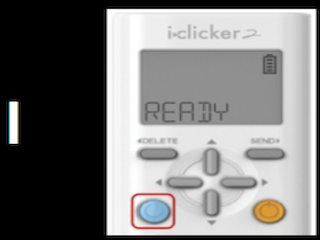
\includegraphics[width=0.3\textwidth]{figures/clicker_self_paced/self_paced_1}
\hspace{1mm}
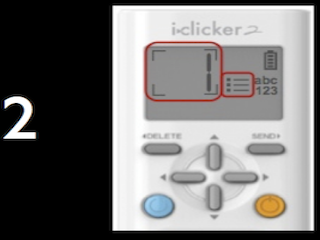
\includegraphics[width=0.3\textwidth]{figures/clicker_self_paced/self_paced_2}
\hspace{1mm}
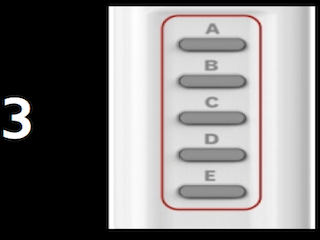
\includegraphics[width=0.3\textwidth]{figures/clicker_self_paced/self_paced_3} \\
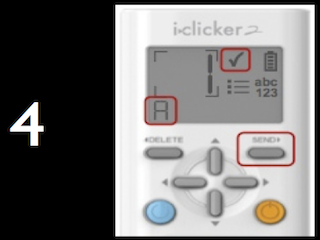
\includegraphics[width=0.3\textwidth]{figures/clicker_self_paced/self_paced_4}
\hspace{1mm}
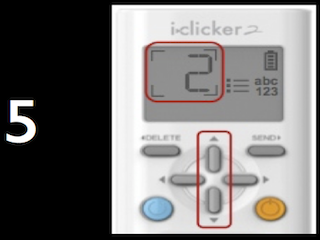
\includegraphics[width=0.3\textwidth]{figures/clicker_self_paced/self_paced_5}
\end{center}

\begin{itemize}

\item \hl{Team:} 10 minutes, using scratch off sheets (1 per team)

\end{itemize}

%---Note---%
\note{

Explain individual RA/clickers:
\begin{itemize}
\item Set frequency (hold down power, click AA).

\item Normally, I'd ask you to put everything away.

\item Normally, 15 minutes, today a little longer.

\item Click on blue button.  You should see square brackets.  Click on A, check
mark.  Your answer has been sent.  Go up down to change question.

\item If you don't see brackets click on blue button.

\item Whether you are registered are not should not matter.

\item You might have questions.  Raise hand and someone will help you.

\item When you are done, turn your clicker over and set it on your desk.

\item Write your name on the piece of paper and circle your answer on the piecen of paper.  This is the only record I will have if we encounter technical difficulties.

\end{itemize}

- Informally put together teams during clicker.
- About 8 minutes in, say if you are done, turn over your clicker.
- Stop once people are done.
- Pause individual portion.

Explain teams/team portion of RA.
\begin{itemize}
\item Normally, you would be with team, today you are with impromptu teams.

\item It would be too hard for everyone to find each other today.  Tomorrow in lab you will be put into teams.

\item I want you to sit with your team in class.

\end{itemize}

Explain scratch sheet:
\begin{itemize}
\item Use doc cam.

\item For the team portion you will use scratch out sheets.

\item Scratch once, if correct good.  Scratch again for second try.

\item 10 minutes for group scratching. (Set up timer.)

\item When you are done, I will pick up your scratch off sheet AND your paper readiness assessment.

\end{itemize}

Give 1 minute warning:
\begin{itemize}
\item You have one minute.

\item When time is up if you haven't given me your scratch off or readiness assessment, walk it up to the front and set it on the table.

\end{itemize}

While the team portion of the RA is going:
\begin{itemize}

\item Write percentage next to each question and circle correct answer.  Usually, pick off two or three questions to go over.

\item pick a couple to go over.

\item read the question back to them.

\item tell the students which learning objectives each question covered.

\end{itemize}

Question 1: types of variables
\begin{itemize}
\item first learning objective: describing variables.

\item question 1: populations can only take on whole numbers.  Can you yave 1000.5 people?

\end{itemize}

Question 5: skewed distributions
\begin{itemize}
\item we want to figure out shape of distribution: symmetric, skewed

\item It really helps to draaw things out.  Use doc cam.  Minimum amount 0:
  boundary.  put 50k marks, try to draw to scale.  What is the total area under
  the curve?  100\%.  Break into quarters.  Are there any natural boundaries?
  Costs, salaries, etc.

\end{itemize}


Question 10: randomization test.
\begin{itemize}

\item Just based on data what is it pointing to?  Are people with pets more less likely to be stressed?

\item But this is just true of sample.  Want to say something about the
entire population.  One method is simulation based method.  Randomization.  Last
video you watched.

\item Total of 40 cards.  18 cards.  Wrote word overstressed on 18.  Shuffle.
Randomly split into two groups of 20.  Do I have any control over how many went
to one group or another.  

\item What would I expect the number to be in each group.

\item What would the expected difference be?  0. 

\item If you expect 0 but you see 2 is that something that is due to chance? What we will learn is whether difference of 2 is statistically significant.  This is what we are learning in this class?  Is this difference surprisingly large?

\end{itemize} 

}

\end{frame}

%%%%%%%%%%%%%%%%%%%%%%%%%%%%%%%%%%%

\section{Housekeeping}

%%%%%%%%%%%%%%%%%%%%%%%%%%%%%%%%%%%

\begin{frame}
\frametitle{Announcements}

\begin{itemize}

\item PS 1 is assigned on the course website, start working on it

\item See email / course website for updated TA office hours -- and start making use of them

\end{itemize}

\end{frame}

%%%%%%%%%%%%%%%%%%%%%%%%%%%%%%%%%%%

\section{Main ideas}

%%%%%%%%%%%%%%%%%%%%%%%%%%%%%%%%%%%

\subsection{Always start your exploration with a visualization}
\label{mi1}

%%%%%%%%%%%%%%%%%%%%%%%%%%%%%%%%%%%

\begin{frame}[fragile]
\frametitle{From a past Sta 101 survey...}

\disc{Do you see anything out of the ordinary?}

\begin{center}
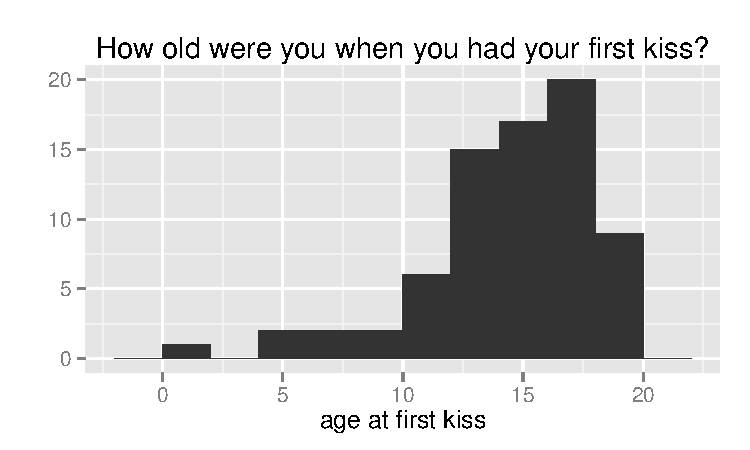
\includegraphics[width=0.8\textwidth]{figures/survey/hist_first_kiss} 
\end{center}

\pause

\soln{Some people reported very low ages, which might suggest the survey
  question wasn't clear: romantic kiss or any kiss?}

%---Note---%
\note{

To day we are going to talk about exploratory data analysis.

- the important thing is to always start your exploratory data analysis with
visualization.

- is there anything out of the ordinary about this?  you probably were first
kissed when you were a baby, but it isn't clear what we are talking about.

- so this is an example of how we need to be careful how we phrase a question.
we want to phrase it so that there is only one interpretation.

}

\end{frame}

%%%%%%%%%%%%%%%%%%%%%%%%%%%%%%%%%%%

\begin{frame}[fragile]
\frametitle{From a past Sta 101 survey...}

\disc{How are people reporting lower vs. higher values of FB visits?}

\begin{center}
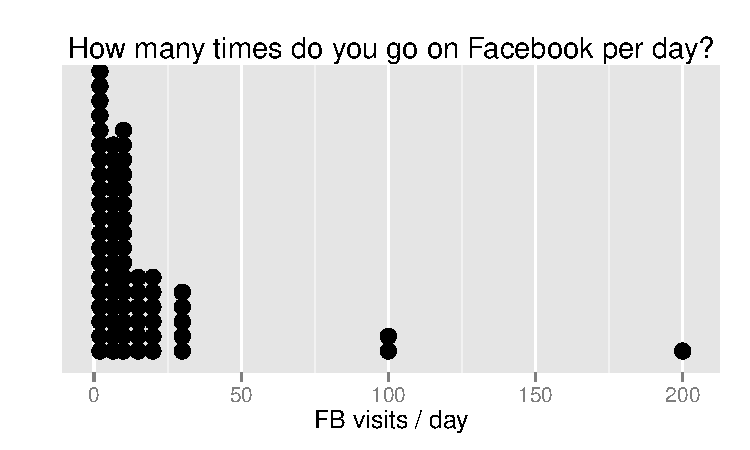
\includegraphics[width=0.8\textwidth]{figures/survey/dot_fb_visits_per_day} 
\end{center}

\pause

\soln{Finer scale for lower numbers.}

%---Note---%
\note{

How many people reporting lower vs. higher values of FB?  It is either 100 or
200, not 107, 113.

We can see that if you don't give guidance on data then it can be tough to
analyze.

}

\end{frame}

%%%%%%%%%%%%%%%%%%%%%%%%%%%%%%%%%%%

\begin{frame}
\frametitle{}

\disc{Describe the spatial distribution of preferred sweetened carbonated beverage drink.}

\begin{center}
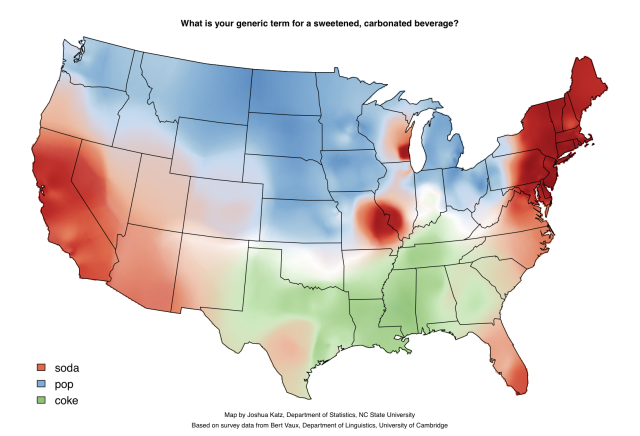
\includegraphics[width=0.9\textwidth]{figures/spatial/soda}
\end{center}

\ct{\webURL{http://spark.rstudio.com/jkatz/SurveyMaps}}

%---Note---%
\note{

How do we refer to these maps?

An intensity map.

Do people call there sweetened carbontated drink pop, etc.

Describe how people do.

Really we are looking at two variables: geographic location and terminology.

}

\end{frame}

%%%%%%%%%%%%%%%%%%%%%%%%%%%%%%%%%%%

\begin{frame}
\frametitle{}

\disc{What is missing in this visualization?}

\begin{center}
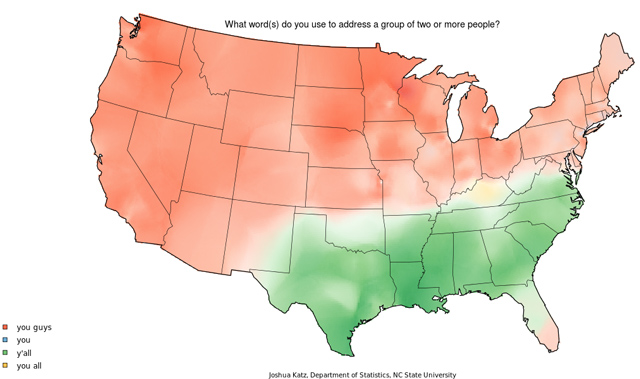
\includegraphics[width=0.9\textwidth]{figures/spatial/yalls}
\end{center}

\ct{\webURL{http://spark.rstudio.com/jkatz/SurveyMaps}}

%---Note---%
\note{

 How do you address a group.

 Describe.

 What do you think is missing in this visualization.

 What would be useful beyond the colors?  What does the shade of the color
 represent?  We have no idea of what value it corresponds to?

 It is missing some information about the numerical intensity that would help us
 compare across colors

 Important point: always start with a visualization.

}

\end{frame}

%%%%%%%%%%%%%%%%%%%%%%%%%%%%%%%%%%

\subsection{When describing numerical distributions discuss shape, center, spread, and unusual observations}
\label{mi2}

%%%%%%%%%%%%%%%%%%%%%%%%%%%%%%%%%%%

\begin{frame}
\frametitle{Describing distributions of numerical variables}

\begin{itemize}

\item \hl{Shape}: skewness, modality

\item \hl{Center}: an estimate of a \hl{typical} observation in the distribution (mean, median, mode, etc.) 
\begin{itemize}
\item Notation: $\mu$: population mean, $\bar{x}$: sample mean
\end{itemize}

\item \hl{Spread}: measure of variability in the distribution (standard deviation, IQR, range, etc.)

\item \hl{Unusual observations}: observations that stand out from the rest of the data that may be suspected outliers

\end{itemize}

%---Note---%
\note{

  Always talk about shape, center, spread, etc.

  Shape

  What do I mean by modality: promenent peaks.

  When talking about center, what is most common measure of center: mean

  What else: median.

  Mode is also used, though it isn't always that useful.  It is the most
  frequent observation.  But it is sometimes hard to determine what that is when
  working with continuous numerical data.

  Just a note for notation: $\mu$ or any greek letter denotes a pop. param.
  $\mu$ is pop bar.

  xbar is a sample statistic.  Often times we want to know mu, but we don't have
  pop, so we caompute xbar and call that best guess.

  how can we put some uncertainty around best guess to refelect that this comes
  from sample and not whole pop.

  when we talk about spread we are talking about variability in the distrbution.

  unusual observations.  sometimes people just remove outliers.  you should not
  do that unless you have good reason to do so, they may convey important information.

}

\end{frame}

%%%%%%%%%%%%%%%%%%%%%%%%%%%%%%%%%%

\begin{frame}
\frametitle{}

\clicker{Which of these is most likely to have a roughly symmetric distribution?}

\begin{enumerate}[(a)]
\item salaries of a random sample of people from North Carolina
\item \solnMult{weights of adult females}
\item scores on an well-designed exam
\item last digits of phone numbers
\end{enumerate}

%---Note---%
\note{

which of the following is mostly likely to have a roughly symmetric
distribution.

things all over the place.  talk to each other and vote again.

let them have a minute.  Make sure to go again whether you changed your answer
or not.

C is now most popular.

if i were to design example that was symmetic, you would be in trouble.  what is
max, what is min.  so what would this look like.  can everyone get 90s and
above.

usually scores on a well designed exam are left skewed.  decent center, but not
at 100.

left or right skewed?

left.

what about b?  some aveerage weight.  Do we expect sampe number to be above and
below?  we don't expect one end to be more frequent than others.

what about random samples of salary from nc.  what we we expect the shape of
that to be?

last digits of phone numbers?  what type of shape might we expect?  there is not
one digit that is more popular than the others.n

}

\end{frame}

%%%%%%%%%%%%%%%%%%%%%%%%%%%%%%%%%%%

\begin{frame}
\frametitle{Mean vs. median}

\clicker{How do the mean and median of the following two datasets compare? \\
$\:$\\
Dataset 1: 30, 50, 70, 90 \\
Dataset 2: 30, 50, 70, 1000
}

\begin{enumerate}[(a)]
\item $\bar{x}_1 = \bar{x}_2$, $median_1 = median_2$
\item \solnMult{$\bar{x}_1 < \bar{x}_2$, $median_1 = median_2$}
\item $\bar{x}_1 < \bar{x}_2$, $median_1 < median_2$
\item $\bar{x}_1 > \bar{x}_2$, $median_1 < median_2$
\item $\bar{x}_1 > \bar{x}_2$, $median_1 = median_2$
\end{enumerate}

%---Note---%
\note{

how do the mean and median of the following compare.  do by yourself first.

give you a minute.

b is the winner.  everyone got it.

% can I explain this in words?

what is the idea we are getting at here?  some extreme value is affecting the
mean, but not the median.  so it is more robust.

}

\end{frame}

%%%%%%%%%%%%%%%%%%%%%%%%%%%%%%%%%%%

\begin{frame}
\frametitle{Standard deviation and variance}

\begin{itemize}

\item Most commonly used measure of variability is the \hl{standard deviation}, which roughly measures the average deviation from the mean
\begin{itemize}
\item Notation: $\sigma$: population standard deviation, $s$: sample standard deviation
\end{itemize}

\item Calculating the standard deviation, for a population (rarely, if ever) and for a sample:

\[ \darkgray{$\sigma = \sqrt{\frac{\sum_{i = 1}^N (x_i - \mu)^2}{n}}$} \qquad s = \sqrt{\frac{\sum_{i = 1}^n (x_i - \bar{x})^2}{n - 1}} \]

\item Square of the standard deviation is called the \hl{variance}.

\end{itemize}

%---Note---%
\note{

spread.  here we are going to go about standard deviation.

one of the more tedious computations.

it roughly measures the average deviation from the mean.

we want to think about how far or how close the data are from the mean on
average.

notation: sigma, greek population standard devaition.  s: sample standard
deviation.

gray here is population data, we rarely have this.

a couple things: used square.  and divide by $n-1$.

why use squares.

standard deviation is nice because it is the same units as what you measure.

}

\end{frame}

%%%%%%%%%%%%%%%%%%%%%%%%%%%%%%%%%%%

\begin{frame}
\frametitle{More on SD}

\disc{Why divide by $n - 1$ instead of $n$ when calculating the sample standard deviation?}

\pause

Lose a ``degree of freedom" for using an estimate (the sample mean, $\bar{x}$), in estimating the sample variance/standard deviation.

\pause

$\:$ \\

\disc{Why do we use the squared deviation in the calculation of variance?}

\pause

\begin{itemize}
\item To get rid of negatives so that observations equally distant from the mean are weighed equally.
\item To weigh larger deviations more heavily.
\end{itemize}

%---Note---%
\note{

why divide by $n-1$ instead of $n$?

go back.  comopare equations.  ideally use population mean.  this introduces
extra uncertatiny.  for that we need to penalize ourselves.

if i divide by $n-1$ or $n$ which yields a higher value?  if i divide by
something smaller, I get a larger number.

so we are in effect reporting a larger estimate of the standard deviation.  this
is conservative.

go forward.  why square things?  what happens if we add a positive and a
negative number?  they cancel out.

one reaons, you don't want poitives and negatives to cancle.

what would be a more intuitive way?

abs.

what does square do?  it weights larger deviations more heavily?

}

\end{frame}

%%%%%%%%%%%%%%%%%%%%%%%%%%%%%%%%%%%

\begin{frame}
\frametitle{Range and IQR}

\clicker{True / False: The range is always at least as large as the IQR for a given dataset.}

\begin{enumerate}[(a)]
\item \solnMult{Yes}
\item No
\end{enumerate}

\soln{\pause Range = max - min, IQR = Q3 - Q1}

$\:$ \\
\pause

\disc{Is the range or the IQR more robust to outliers?}

\soln{\pause{IQR}}

%---Note---%
\note{

Give about 45 seconds.

many yeses some nos.  can i hear from someone that said no?

what is definition of iqr.

what is definition of range.

is the range or iqr more robust to iqr robust to outliers?  outliers are most
likely minimum or maximum points.  calculation of range is based on exactly
these values.


}

\end{frame}

%%%%%%%%%%%%%%%%%%%%%%%%%%%%%%%%%%%

\subsection{Robust statistics are not easily affected by outliers and extreme skew}
\label{mi3}

%%%%%%%%%%%%%%%%%%%%%%%%%%%%%%%%%%%

\begin{frame}
\frametitle{Robust statistics}

\begin{itemize}

\item Mean and standard deviation are easily affected by extreme observations since the value of each data point contributes to their calculation.

\item Median and IQR are more robust.

\item Therefore we choose median\&IQR (over mean\&SD) when describing skewed distributions.

\end{itemize}

%---Note---%
\note{

median and iqr are robust.  this is why use them do describe skewed
distribution.

which is more informative for skewed distribution?

when describing dist, first think about shape, then think about numbers to use
to describe.

it is on you to get an idea on visualization and then pick.


}

\end{frame}

%%%%%%%%%%%%%%%%%%%%%%%%%%%%%%%%%%%

\subsection{Use box plots to display quartiles, median, and outliers}
\label{mi4}

%%%%%%%%%%%%%%%%%%%%%%%%%%%%%%%%%%%

\begin{frame}
\frametitle{Box plot}

A \hl{box plot} visualizes the median, the quartiles, and suspected outliers. An \hl{outlier} is defined as an observation more than 1.5$\times$IQR away from the quartiles.

\begin{center}
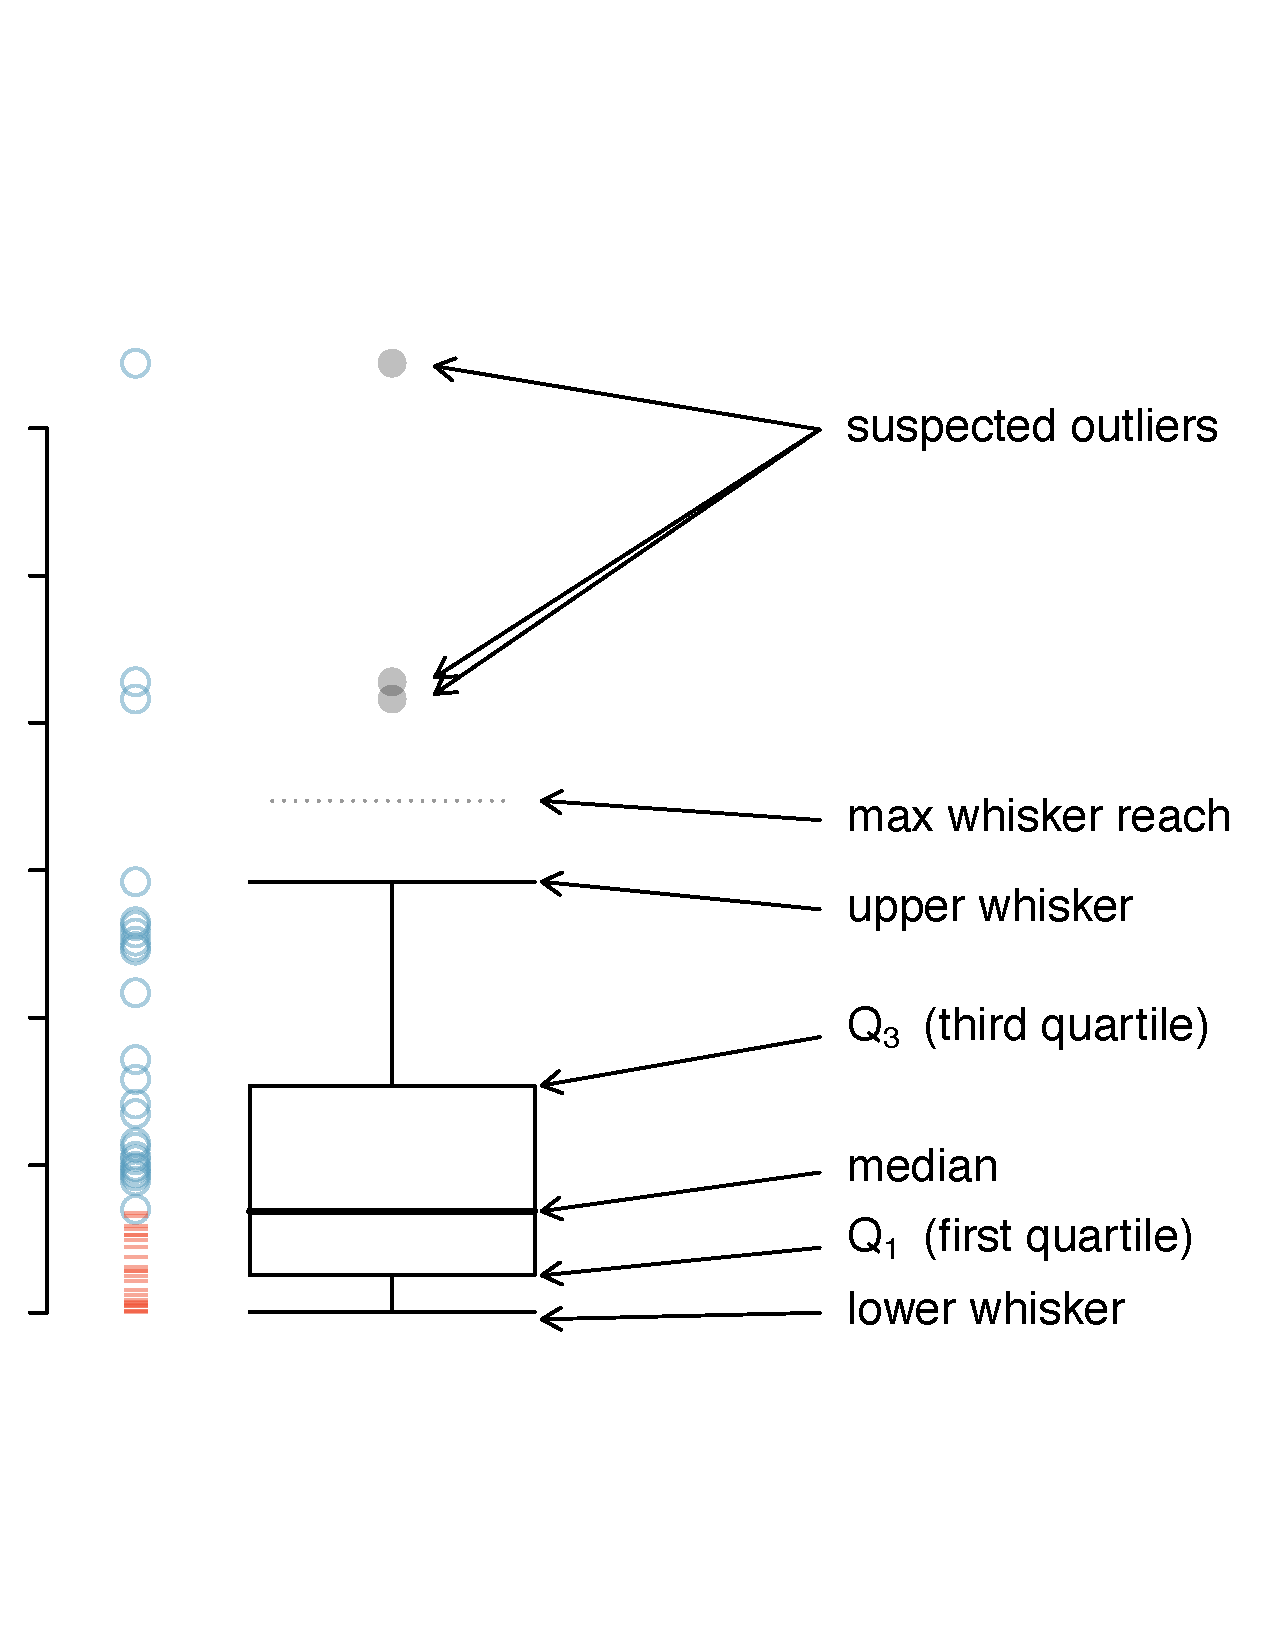
\includegraphics[width=0.6\textwidth]{figures/boxPlotLayoutNumVar}
\end{center}

%---Note---%
\note{

boxplot is useful for median, iqr.

data set of 5, where will the median be.

if 6, where will it be?

boxplots are good for showing where outliers are.

fence: 1.5 iqr.

explain whiskers.  whiskers are 1.5 from interquartile range.

}

\end{frame}

%%%%%%%%%%%%%%%%%%%%%%%%%%%%%%%%%%%

\section{Application exercises}

%%%%%%%%%%%%%%%%%%%%%%%%%%%%%%%%%%%

\begin{frame}
\frametitle{}

\vfill

\app{1.1 Distributions of numerical variables}{$\:$\\ See the course website for instructions. \\$\:$}

\vfill

%---Note---%
\note{

you get 10 minutes to work on in teams.

randomly pick a team to discuss answers on board.

make sure you are concise, but clear.

1. 

a: digits
b: marriage

2. 

a: 2
b: 1 why 1 and not 4?
c: 6: right skewed
d: 3: a few people pulling all nighters
e: 4: on campus
f: 5: what do we think the numbers are?  what are most common?

3. think about numerical/categorical (are we looking at bar plot or histogram);
think about natural boundaries---there is a lower bound on piercings; then think
about shape: skew, symmetry, think about the modes.

4. Need to actually compute.

team claimed, a, c, b for variability.

Be careful about explain your reasoning.

5. E is more variable. 

Be careful about explain your reasoning.  more values that are closer to the
mean.

variability vs diversity.  diversity is not smooth.

Ask if people need more time.  Tell people they are welcome to go onto next app
ex if they are done.

Make sure you go ahead and submit your responses.

state names.

}

\end{frame}

%%%%%%%%%%%%%%%%%%%%%%%%%%%%%%%%%%%%

\section{Summary}

%%%%%%%%%%%%%%%%%%%%%%%%%%%%%%%%%%%%

\begin{frame}
\frametitle{Summary of main ideas}

\vfill

\begin{enumerate}

\item \nameref{mi1}

\item \nameref{mi2}

\item \nameref{mi3}

\item \nameref{mi4}

\end{enumerate}

\vfill

\end{frame}

%%%%%%%%%%%%%%%%%%%%%%%%%%%%%%%%%%%

\end{document}